
\begin{figure}[htbp]
\label{fix:exp-results}
  \centering

  \begin{subfigure}[b]{0.45\textwidth}
    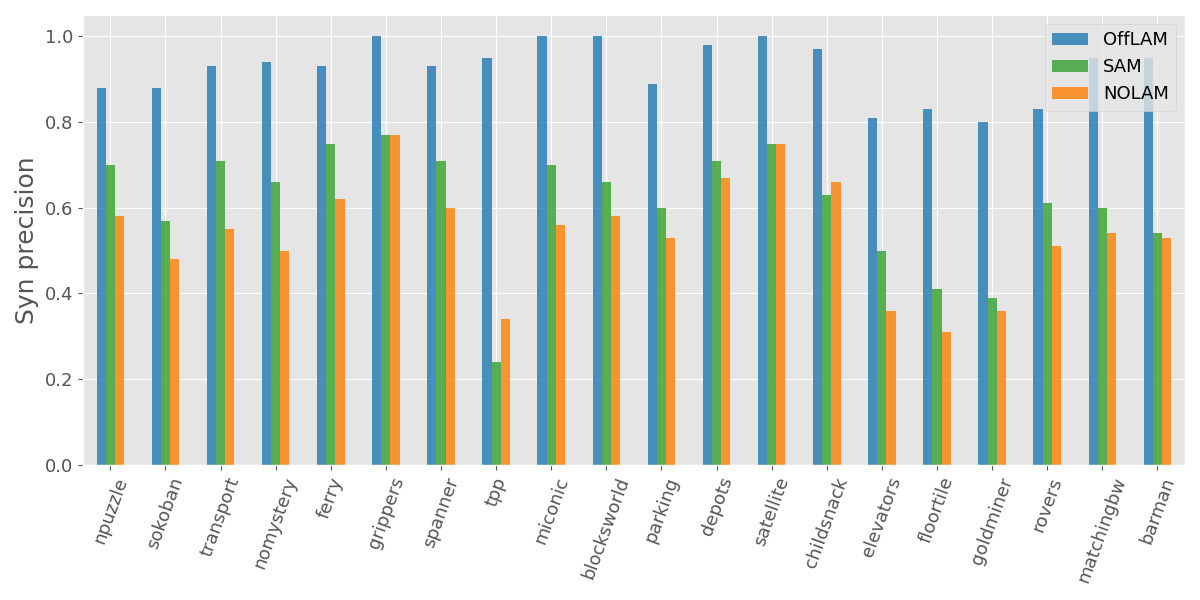
\includegraphics[width=\textwidth]{figures/syn_precision.png}
    \caption{Syntactic precision}
  \end{subfigure}
  \hfill
  \begin{subfigure}[b]{0.45\textwidth}
    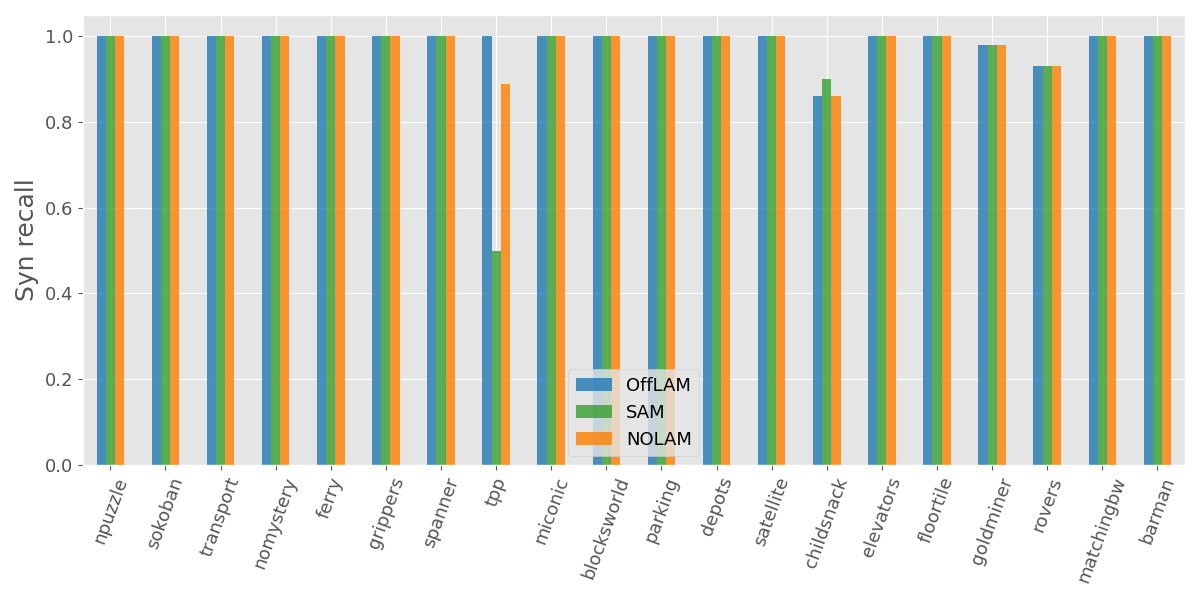
\includegraphics[width=\textwidth]{figures/syn_recall.png}
    \caption{Syntactic recall}
  \end{subfigure}

  \vspace{1em}

  \begin{subfigure}[b]{0.45\textwidth}
    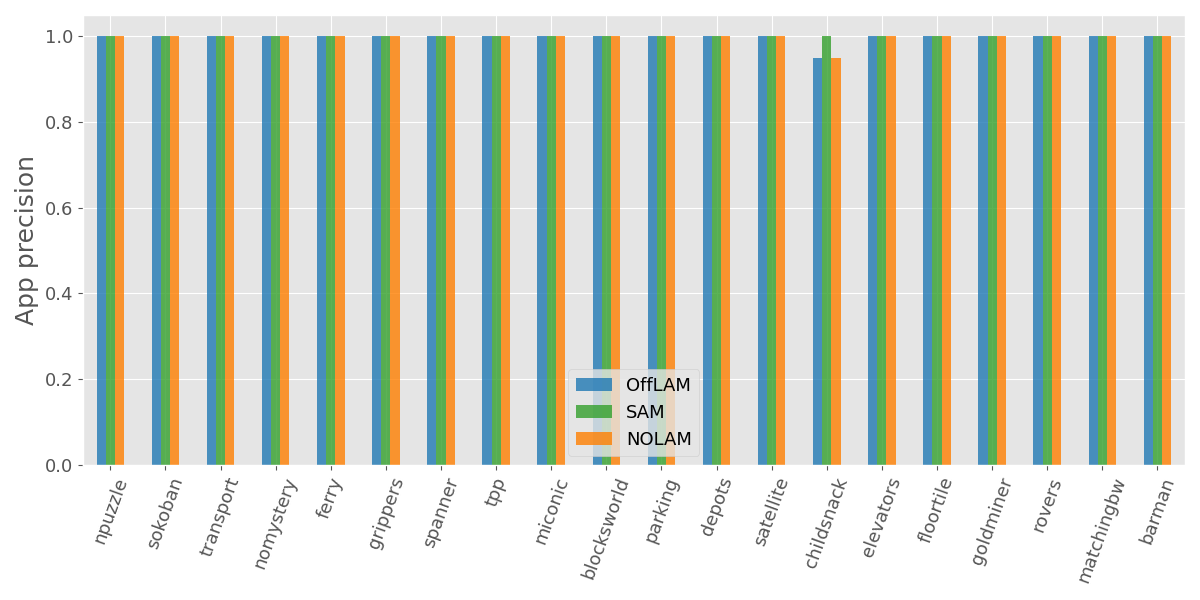
\includegraphics[width=\textwidth]{figures/app_precision.png}
    \caption{Applicability precision}
  \end{subfigure}
  \hfill
  \begin{subfigure}[b]{0.45\textwidth}
    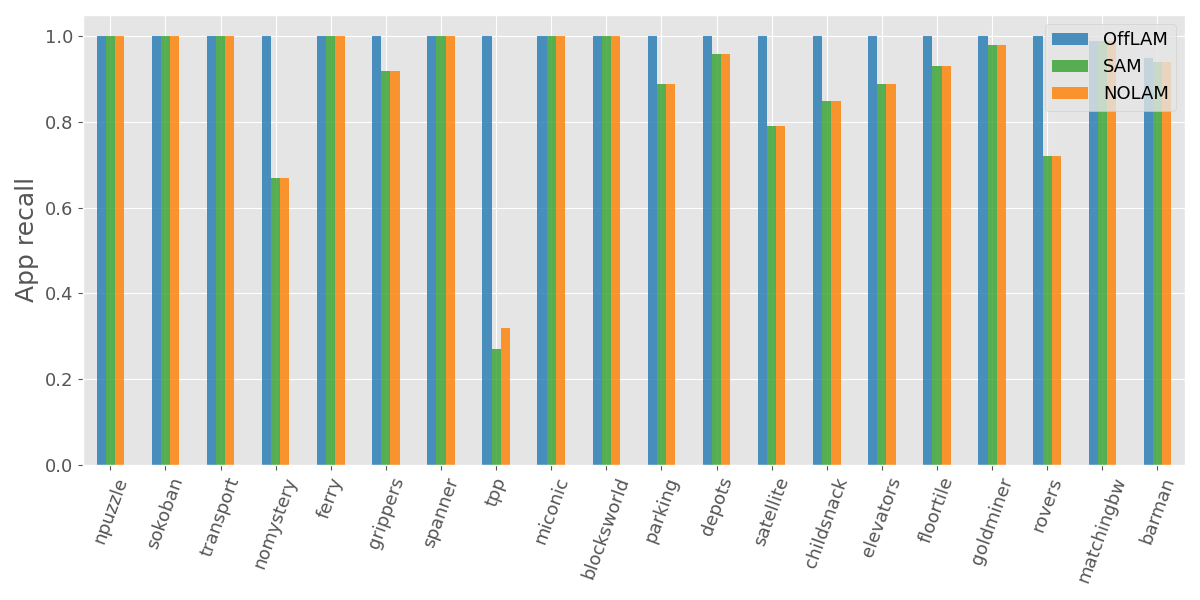
\includegraphics[width=\textwidth]{figures/app_recall.png}
    \caption{Applicability recall}
  \end{subfigure}

  \vspace{1em}

  \begin{subfigure}[b]{0.45\textwidth}
    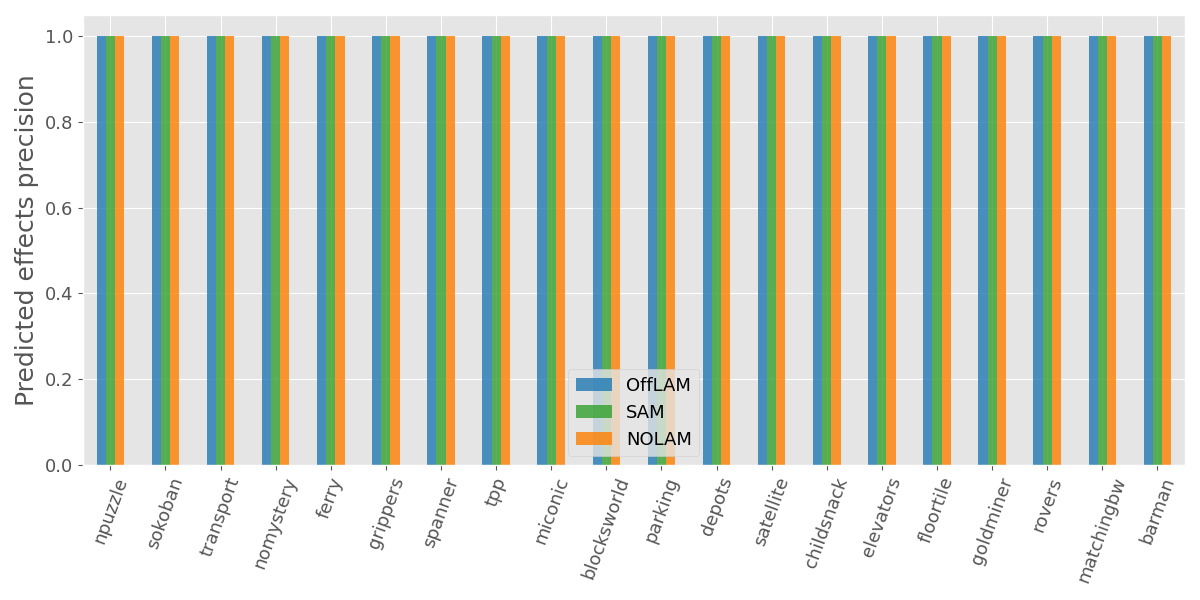
\includegraphics[width=\textwidth]{figures/predeffs_precision.png}
    \caption{Predicted effects precision}
  \end{subfigure}
  \hfill
  \begin{subfigure}[b]{0.45\textwidth}
    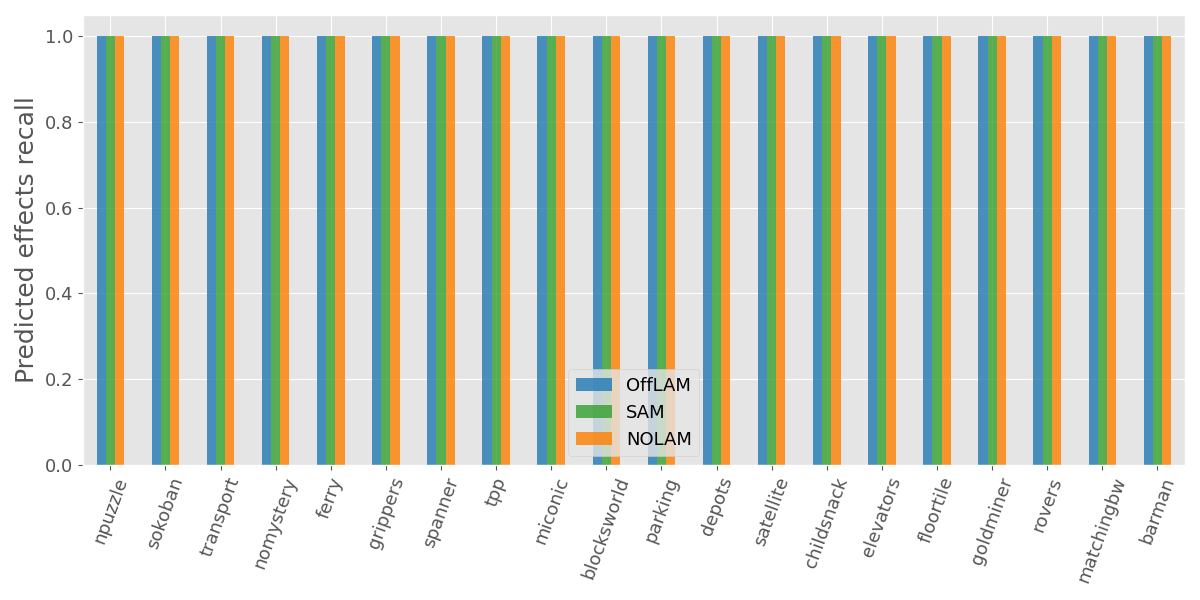
\includegraphics[width=\textwidth]{figures/predeffs_recall.png}
    \caption{Predicted effects recall}
  \end{subfigure}

  \vspace{1em}

  \begin{subfigure}[b]{0.45\textwidth}
    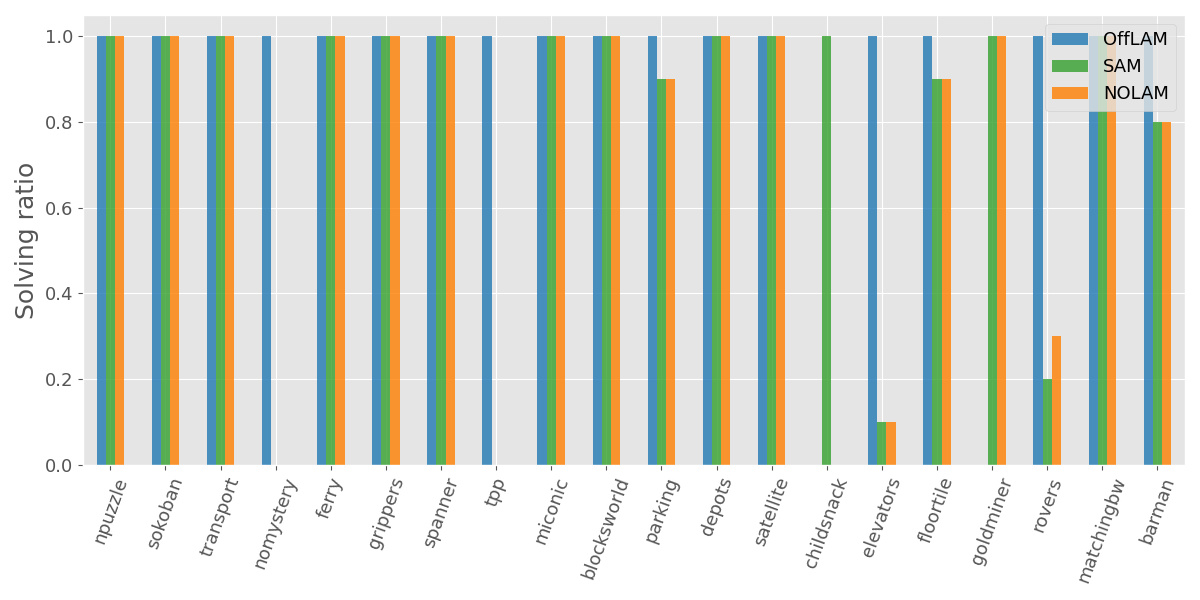
\includegraphics[width=\textwidth]{figures/solving.png}
    \caption{Problem solving ratio}
  \end{subfigure}
  \hfill
  \begin{subfigure}[b]{0.45\textwidth}
    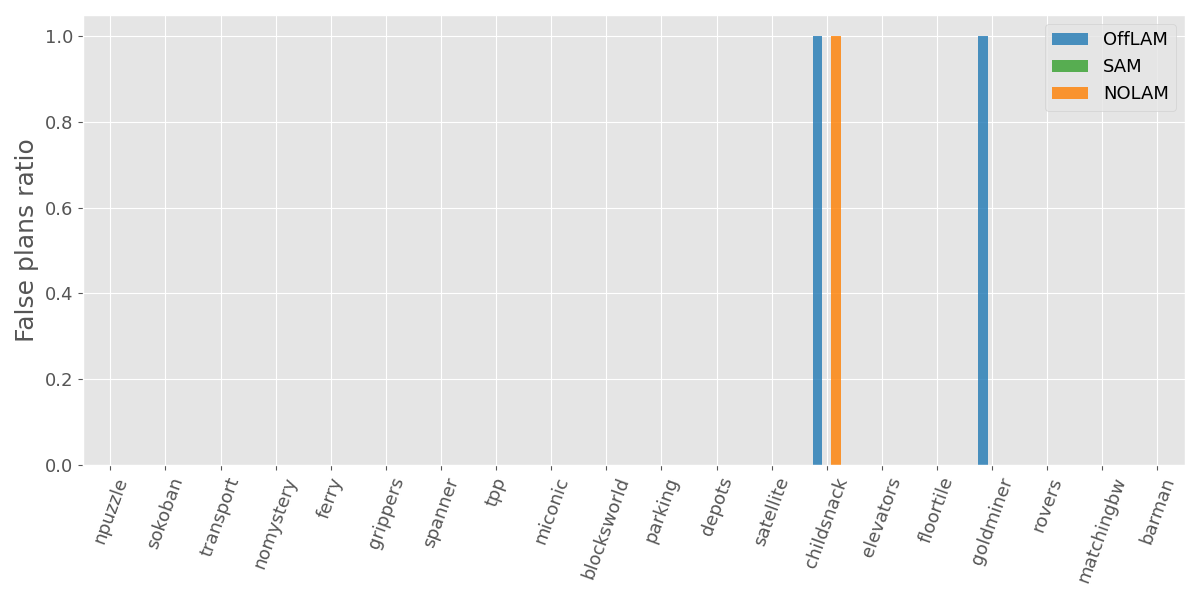
\includegraphics[width=\textwidth]{figures/false_plans.png}
    \caption{False plans ratio}
    \label{fig:false-positive-plans}
  \end{subfigure}

  % \caption{Overall caption for the 6 images.}
  \label{fig:exp}
\end{figure}